\chapter{Rešerše dostupných řešení}

Cílem této kapitoly je provést průzkum existujících nástrojů pro licencování
aplikací s cílem zmapování poskytované funkcionality. Hlavní důraz při hodnocení
je kladen na následující vlastnosti:

\begin{itemize}
  \item Integrovatelnost s aplikacemi napsanými v jazyce Java
  \item Podpora pro aplikace napsané na platformě Eclipse/OSGi
  \item Funkčnost v operačních systémech Linux a Windows
  \item Možnost centrální správy licencí
  \item Možnost vázat licenci na konkrétní hardware
  \item Cena řešení 
\end{itemize}


\section{License4j}

License4j\cite{license4j} je jendoduchá knihovna, která umožňuje vytvářet
licence pro aplikace napsané v Javě. Obsahuje GUI nástroj pro generování
licenčních souborů, které se digitálně podepíší a přibalí se k výsledné
aplikaci. Platnost souboru se kontroluje v aplikaci pomocí přidaného veřejného
klíče, čímž je znemožňeno modifikovat licenční soubor.

\begin{figure}[H]
\begin{center}
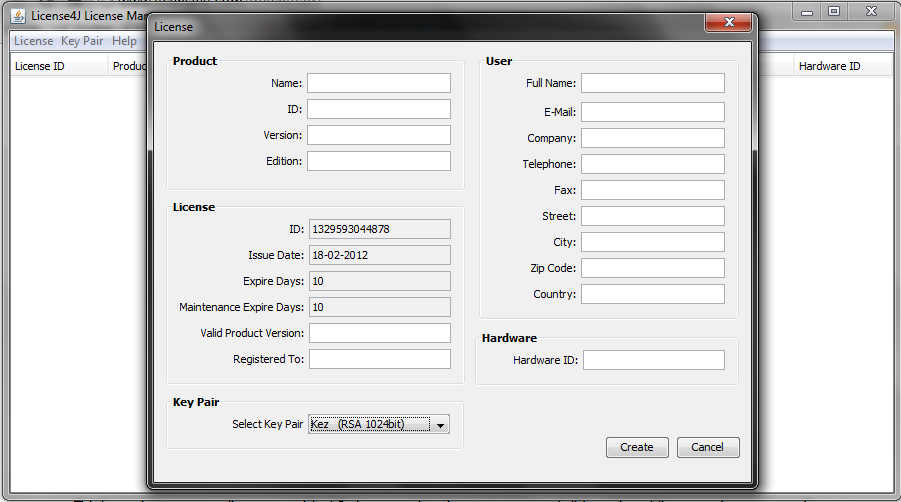
\includegraphics[width=12cm]{figures/license4j.PNG}
\caption{License4j UI pro tvorbu licencí}
\label{fig:license4j-ui} 
\end{center}
\end{figure}

\subsection*{Vlastnosti}
Aplikace je dostupná volně ke stažení, verze zdarma umožňuje vytvářet licence s
platností 10 dní, licenci pro plnou funkčnost je možné zakoupit za částku \$35.
K produktu je navíc možné dokoupit roční rozšířenou podporu za \$15.

Distribuovaná verze obsahuje knihovny a GUI bez zdrojových kódů. Mezi vlastnosti
produktu patří:

\begin{itemize}
  \item Ruční výroba licenčního souboru pomocí dodané aplikace s GUI,
  předdefinované položky v licenci
  \item Možnost zabudování MAC adresy nebo hostname do licenčního souboru
  \item Kontrola platnosti licence za běhu pomocí veřejného klíče 
\end{itemize}

\subsection*{Zhodnocení}
License4j je jendoduchoá knihovna s velmi omezeným použitím, čemuž odpovídá i
poměrně nízká pořizovací cena. 

Výhodou může být snadná integrovatelnost s existujícími aplikacemi a snadná
výroba licenčních klíčů pomocí dodaného GUI.

Hlavní nevýhodou tohoto produktu je potřeba ručně generovat licenční soubory
pro každého zákazníka, což může být při distribuci většího množství licencí
problematické. Licence je sice možné vázat na MAC adresu nebo hostname, to ale
není pro reálné použití příliš vhodné.


\section{JLicense}
Podobně jako u předchozího produktu se v případě JLicense\cite{jlicense} jedná o
jednoduchou knihovnu, která umožňuje pomocí GUI generovat licenční klíče,
jejichž platnost se poté v aplikaci kontroluje pomocí digitálního podpisu.

\begin{figure}[H]
\begin{center}
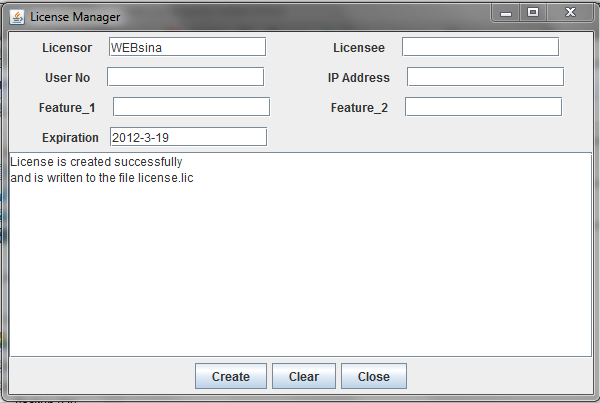
\includegraphics[width=12cm]{figures/jlicense.PNG}
\caption{JLicense UI pro tvorbu licencí}
\label{fig:jlicense-ui} 
\end{center}
\end{figure}

\subsection*{Vlastnosti}
Knihovnu je možné stáhnout a používat zdarma. V případě zájmu je možné koupit
zdrojové kódy za cenu \$50. Vlastnosi produktu jsou:

\begin{itemize}
  \item Ruční výroba licenčního souboru pomocí dodané aplikace s GUI,
  předdefinované položky v licenci
  \item Možnost zabudování IP adresy do licence
\end{itemize}

\subsection*{Zhodnocení}
Jedná se o produkt funkčně shodný s knihovnou License4j. Výhodou může být
možnost neomezeného použití zdarma a také dostupnost zdrojových kódů za
poplatek.


\section{Rampart}
Posledním ze zástupců kategorie malých knihoven je knihovna
Rampart\cite{rampart}. Stejně jako v předchozích připadech se produkt skládá z
GUI pro generování licenčních souborů a runtime knihovny pro ověřování
vygenerovaných licencí.

\begin{figure}[H]
\begin{center}
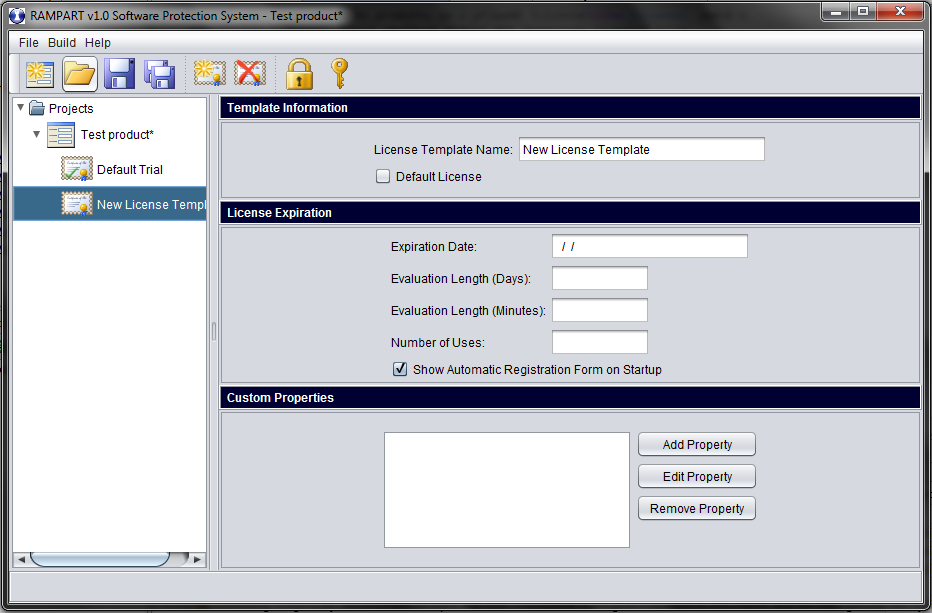
\includegraphics[width=12cm]{figures/rampart.PNG}
\caption{Rampart UI pro tvorbu licencí}
\label{fig:rampart-ui} 
\end{center}
\end{figure}

\subsection*{Vlastnosti}
Trial verzi s omezenou platností na 30 dní je možné zdarma stáhnout z webových
stránek výrobce, licenci na plnou verzi je možné zakoupit za \$29. Mezi
vlastnosti produktu patří:

\begin{itemize}
  \item Výroba a správa licencí pomocí GUI
  \item Podpora pro trial verze
\end{itemize}

\subsection*{Zhodnocení}
Výhodou tohoto produktu oproti předchozím je mnohem propracovanější nástroj pro
správu licencí. Runtime knihovna také umožňuje zobrazovat dialogy usnadňující
získání licence.

nevýhodou může být fakt, že vydané licence není možné jakkoliv vázat na
hardware.

\section{Protection! 4}

Produkt Protection! 4\cite{protection} je první ze zkoumaných produktů přímo
určený pro nasazení v enterprise prostředí. Obsahuje jak velmi pokročilý nástroj
umožňující vytváření, správu a integraci licencí, tak i server pro centrální
správu licencí.

\begin{figure}[H]
\begin{center}
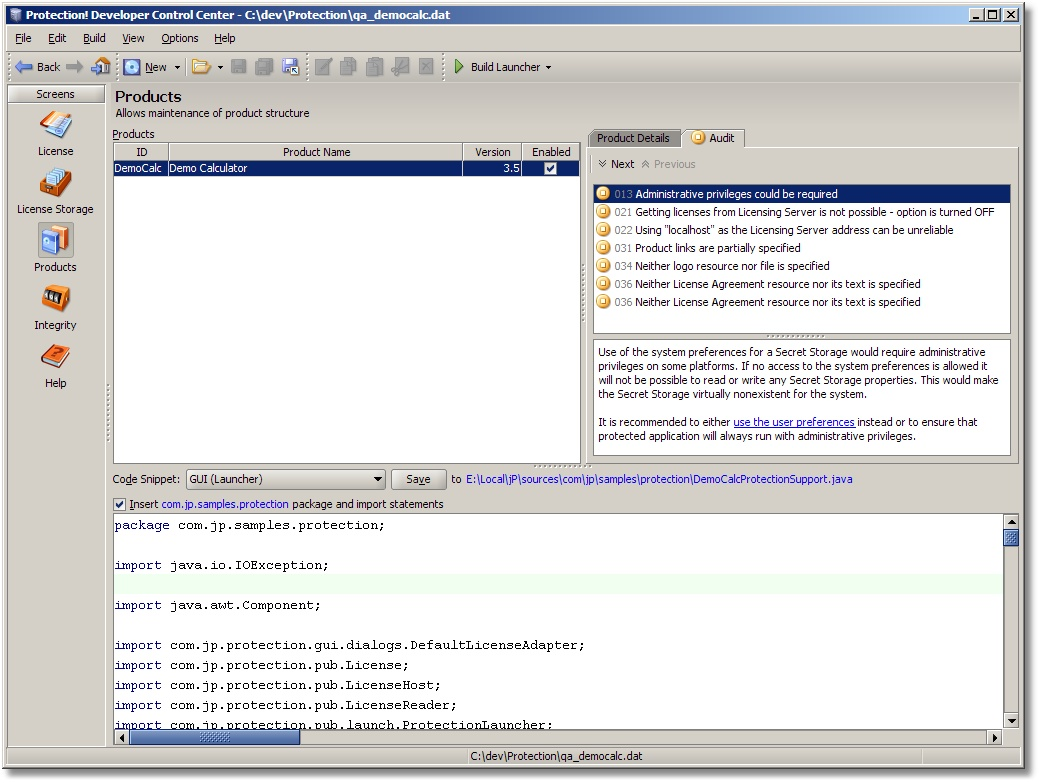
\includegraphics[width=12cm]{figures/protection4.PNG}
\caption{Protection developer control center}
\label{fig:protection4-ui} 
\end{center}
\end{figure}

\subsection*{Vlastnosti}
Jendá se o ryze komerční řešení, ze stránek výrobce se dají stáhnout všechny
potřebné nástroje, je ale potřeba kontaktovat výrobce ohledně vystavení trial
licence. Cena je \$997 za licenci pro desktopovou aplikaci pro jednoho
vývojáře, serverový backend stojí \$5000 na rok na jedno procesorové jádro. Je
možné také dokoupit dodatečnou podporu.

\begin{itemize}
  \item Výroba a správa licencí pomocí pokročilého grafického nástroje
  \item Grafický nástroj usnadňující integracio ochrany do aplikace vytvářející
  vlastní launcher
  \item Podpora pro trial verze
  \item Webová služba umožňující integraci s existujícími systémy
  \item Možnost vázat licenci na hardware počítače
  \item Licenční server včetně webového rozhraní pro správu licencí
  \item Možnost vydávat licence vázané na hardware i licence omezené počtem
  souběžně běžících kopií
  \item Kontrola integrity aplikace pro znesnadnění odstranění ochrany
\end{itemize}

\subsection*{Zhodnocení}
Jedná se o pokročilé řešení určené pro větší podniky s velkým množstvím
vlastností. Nevýhodou může být vysoká pořizovací cena pro menší projekty.

\section{LM-X License Manager}
LM-X License Manager\cite{lm-x} je další z komerčních licenčních nástrojů
orientovaný na velké společnosti. Produkt je distribuován v podobě SDK napsaného
v C++, pro integraci s aplikacemi napsanými v Javě výrobce poskytuje obalovací
třídy.

\subsection*{Vlastnosti}
Výrobce umožňuje stažení testovací verze s omezenou dobou platnosti zdarma po
vyplnění kontaktního formuláře. Platnost testovací verze je možné prodloužit za
poplatek \EUR{200} na 3 měsíce. Cena licence pro komerční použití závisí na
obratu společnosti a počtu platforem. Nejlevnější licence pro společnost s
obratem pod \EUR{1M} vyjde na \EUR{1500} za rok a \EUR{550} za každou další
platformu.

Vlastnosti produktu:

\begin{itemize}
  \item Integrace s aplikacemi pomocí výrobcem dodaného SDK
  \item Možnost vystavovat licence vázané na hardware i plovoucí licence
  \item Licenční server pro centrální správu licencí 
\end{itemize}

\subsection*{Zhodnocení}
Opět se jedná o profesionální licenční řešení, takže jeho hlavní výhodou je
velké množství funkcí a podpora od výrobce.

Jako nevýhoda se kromě ceny může také jevit skutečnost, že dodávaná knihovna je
napsaná v C++ a pro použití s aplikacemi napsanými v Javě je potřeba používat
obalovací třídy. K aplikaci je tedy nutné přibalit i zkompilované knihovny pro
každou podporovanou platformu.

\section{Vyhodnocení}
Výsledky zkoumaných řešení jsou shrnuty v následující tabulce:

\begin{table}\centering
	\caption[Results]{Porovnání hodnocených produktů}\label{tab:research-results}
	\begin{tabular}{|p{2cm}|p{4cm}|l|p{4cm}|}\hline
		Název			& Podporované platformy	& Podpora Eclispe/OSGi	& Cena
		\tabularnewline \hline \hline 
		License4j		& Java					& Ne					& \$35		
		\tabularnewline \hline
		JLicense		& Java					& Ne					& Zdarma, \$50 za zdrojov0 kódy
		\tabularnewline \hline
		Rampart			& Java					& Ne					& \$29
		\tabularnewline \hline
		Protection! 4	& Java					& Ne					& \$997 za vývojáře, \$5000 za serverovou
		část na rok 
		\tabularnewline \hline
		LM-X License Manager & Windows, Linux, MacOS, AIX, Solarix,\ldots & Ne & Dle
		obratu firmy, minimálně \EUR{1500} na rok + \EUR{550} za platformu
		\tabularnewline \hline
	\end{tabular}
\end{table}

Průzkum ukazuje, že dostupná řešení se dělí ve své podstatě na 2 kategorie:

\begin{itemize}
  \item Malé knihovny – poskytují pouze základní funkcionalitu v podobě
  vytváření licencí pomocí dodaného nástroje a knihovnu pro ověřování platnosti
  licence za běhu licencované aplikace. V případě, že nehledáme příliš
  sofistikované řešení může být jejich použití vhodné, obzvláště pak s
  přihlédnutím k ceně. Ta se pohybuje v rozmezí několika desítek dolarů.
  \item Komerční řešení – produkty určené k použití v enterprise prostředí.
  Vynikají především množstvím poskytované funkcionality – od vystavování trial
  licencí, přes licence vázané na hardware až po serverová řešení pro distribuci
  licencí. Tomu ovšem také odpovídá cena, která se pohybuje v řádu tísíců
  dolarů, často s nutností připlácet za další vývojáře, platformy a také za
  každoroční obnovení licence.
\end{itemize}

Ukazuje se také, že žádný z dostupných nástrojů neobsahuje podporu pro aplikace
psané na platformě Eclipse, případně OSGi.
% License4J - http://www.license4j.com/
% - v podstate jen podepsani licencnich udaju + GUI
% - cena = $35
% - generovani HW otisku
%   - mac 
%   - hostname
% - licence se generuje pomoci swingove aplikace
% - do aplikace se zabudujuje verejny klic, overuje se licence
% 
% 
% jProductivity Protection!
% - cena $997 per developer and backend $5,000 per year; per CPU 
% - server + klient reseni
% 
% JLicense - http://www.websina.com/products/jlicense.html#
% - podobne jako License4J
% - cena = $50
% - IP adressa, MAC adresa, User number
% 
% http://www.jproductivity.com/products/protection/protection.htm
% 
% Rampart
% - vytvoreni podepsaneho licencniho souboru, ktery se kontroluje
% - neumoznuje vazbu na HW
% - cena $29


%LM-X
%- 1500
